\documentclass[twocolumn,amsmath,amssymb,pra]{revtex4-2}
\usepackage[utf8]{inputenc}
\usepackage{amsmath}
\usepackage{graphicx}
\graphicspath{ {figures/} }
\usepackage{siunitx}
\usepackage{hyperref}
\usepackage{float}


\begin{document}

\title{Physics 357-0: Quantum Optics}

\author{Jun Sung, Darren Ding, Ivan Fithian}

\date{12/07/21}

\maketitle

\section{Introduction}
For most students who have a basic background in physics, they are often led to believe that the photoelectric effect and Compton scattering are proofs for light being made up of photons; this is simply not true, though, as both strongly suggest the existence of photons, they do not demand it. In order to prove that photons exist, it suffices to devise an experiment whose result cannot be explained using a classical wave theory of light. In this lab, we shall prove the existence of photons by repeating the experiment devised by Grangier, Roger, and Aspect. Furthermore, we shall also study the quantum mechanical nature of light by disproving the Hidden Variable Theory (HVT) by violating the Bell inequality.

\subsection{Basic Overview of Methods}
This lab consists of two main parts: 
\begin{itemize}
    \item Calculating the second-order coherence $g^{(2)}(0)$
    \item Seeing if we can violate the Bell inequality -- that is, seeing if we can obtain a measurement of $S > 2$
\end{itemize}
For the first part, we shall repeat the experiment that Grangier, Roger, and Aspect performed as mentioned earlier; their approach was to examine and measure correlations between photodetections at the transmission and reflection outputs of a 50/50 beamsplitter. The thought was that if a single quantum of light is incident on the beamsplitter, then it should be detected at the transmission output or at the reflection output, but not both -- i.e., there should be no coincident detections between the two outputs. We then use these measurements to calculate the degree of second-order coherence, which will then tell us whether or not the field incident on the beamsplitter was well described by the QM descriptions of a field in a single photon state.

For the second part, we use half-waveplate polarizers (HWP) set at specific angles to obtain the same type of measurements that we made for the first part of the lab. From these measurements, we are able to calculate the corresponding value of $S$ using Eqns. \ref{eq:E_num} and \ref{eq:S}, which will then tell us whether or not our equivalent Bell inequality is violated.

\subsection{Applications}
Quantum optics deals with the application of QM to phenomena involving light and its interactions with matter \cite{picoquant}. In particular, we see that such applications include quantum communication and computing -- both of which are gaining more and more interest. For example, many major companies (such that Google and IBM) are investing resources into building quantum computers. These quantum computers encode information as quantum bits (i.e., qubits), which can be implemented in a variety of ways -- one of them being through the use of photons. However, it should be noted that the quantum computers built by such major companies implement qubits through the use of superconducting circuits.

As for quantum communication, one of the main areas of interest here deals with quantum cryptography. The most well known and developed application of quantum cryptography is quantum key distribution (QKD), which describes the use of quantum mechanical effects to perform cryptographic tasks or to break cryptographic systems \cite{picoquant}. Quantum optics plays a role in this as it allows for one to generate true randomness, which is one important component of virtually all proper encryption schemes.

\section{Theory}

\subsection{Classical Fields}
A classical field is an electromagnetic wave that is perfectly described by Maxwell's equations. For such a field, the correlations between the intensities of the transmitted $I_{T}$ and reflected $I_{R}$ beams are given by the degree of second-order coherence, denoted as $g_{T, R}^{( 2 )} (\tau)$, which is a function of the time delay $\tau$ between the intensity measurements and is of the following:
\begin{equation}
    g_{T, R}^{( 2 )} (\tau)
    =
    \frac{ \langle I_{T}( t + \tau ) I_{R}( t ) \rangle }
    { \langle I_{T}( t + \tau ) \rangle \langle I_{R}( t ) \rangle }
    \label{eq:g_TR_classical}
\end{equation}
With this, we now focus our attention to the case of simultaneous (that is, $\tau = 0$) intensity measurements. If we assume that we are using a 50/50 beamsplitter, then we have that the transmitted, reflected, and incident intensities are related by $I_{T}(t) = I_{R}(t) = \frac{1}{2} I_{I}(t)$. With this case and assumption, we see that Eqn. \ref{eq:g_TR_classical} updates to be 
\begin{equation}
    g_{T, R}^{( 2 )} (0)
    =
    g_{I, I}^{( 2 )} (0)
    =
    \frac{ \langle [ I_{I}(t) ]^{2} \rangle }
    { \langle I_{I}(t) \rangle^{2} }
    =
    g^{( 2 )} (0)
    \label{eq:g_classical}
\end{equation}
If we now utilize the Cauchy-Schwartz inequality, which tells us that $\langle I_{I}(t) \rangle^{2} \leq \langle [ I_{I}(t) ]^{2} \rangle$, then we find that 
\begin{equation}
    g_{T, R}^{( 2 )} (0)
    =
    g^{( 2 )} (0) 
    \geq 1
    \label{eq:ineq_classical}
\end{equation}
We emphasize that the result shown in Eqn. \ref{eq:ineq_classical} was derived using classical wave theory.

\subsection{Semiclassical Theory of Photodetection}
Although we have been speaking about correlations between the intensities of the field leaving the beamsplitter, one does not measure the intensity directly in an experiment; rather, one measures the photocurrent from a detector. Thus, it is necessary to talk about and model the photodetection process.

Since our discussion thus far has been with classical fields, we shall use a model that treats the field classically. In particular, we shall delve into the semiclassical theory of photoelectric detection, where the field is treated classically, while the photodetector is treated quantum mechanically. For the sake of this discussion, it is convenient to refer to the detector monitoring the transmitted and reflected fields as detector $T$ and $R$, respectively. 

In the theory of semiclassical theory of photoelectric detection, it is found that the conversion of continuous electromagnetic radiation into discrete photoelectrons is a random process; we have the probability of obtaining a single photocount from a single detector (say, detector $T$) within a short time window $\Delta t$ is proportional to the average intensity of the field striking that detector -- that is, if we have $\eta_{T}$ to be a constant that characterizes the detection efficiency of detector $T$, then we have 
\begin{equation}
    P_{T}
    =
    \eta_{T} \langle I_{T}(t) \rangle
    \label{eq:P_T}
\end{equation}
Furthermore, we have the joint probability of obtaining a photocount (within a small time window $\Delta t$) at detector $R$, and then obtaining a photocount at detector $T$ (within a small time window $\Delta t$) after a time $\tau$ is given by the following: 
\begin{equation}
    P_{TR} (\tau)
    =
    \eta_{T} \eta_{R} 
    \langle I_{T}(t + \tau) I_{R}(t) \rangle
    \label{eq:P_TR}
\end{equation}
From here, we see that Eqn. \ref{eq:g_TR_classical} can be rewritten in terms of the probabilities $P_{T}$, $P_{R}$, and $P_{TR}$ as follows: 
\begin{equation}
    g_{T, R}^{( 2 )} (\tau)
    =
    \frac{ P_{TR}(\tau) }{ P_{T} P_{R} }
\end{equation}
Again, we now focus our attention to the case of simultaneous (that is, $\tau = 0$) detection of photocounts at detectors $T$ and $R$, which occurs with probability $P_{TR}(t)$. Using the same reasoning mentioned in the Classical Fields sections, we have that 
\begin{equation}
    g_{T, R}^{( 2 )} (0)
    =
    \frac{ P_{TR}(0) }{ P_{T} P_{R} }
    =
    g^{( 2 )} (0) 
    \geq 1
    \label{eq:ineq_semiclassical}
\end{equation}

In summary, we have that it is possible to measure $g^{(2)}(0)$ by measuring $P_{TR}$, $P_{T}$, and $P_{R}$, and it must be the case that $g^{(2)}(0) \geq 1$ for a classical field. Furthermore, since we have that $g^{(2)}(0)$ cannot be less than 1, we are left with the conclusion that the measured photocounts at detectors $T$ and $R$ cannot be anticorrelated. This agrees with the fact that a beamsplitter splits a classical input field into two identical copies; these output fields either fluctuate together (which corresponds to positive correlation, or when $g^{(2)}(0) > 1$) or do not fluctuate at all (which corresponds to no correlation, or when $g^{(2)}(0) = 1$) -- i.e., it is impossible for the intensity of one to decrease while the intensity of the other increases (which corresponds to anticorrelation).

\subsection{Quantum Fields}
We now shift our focus to quantum fields, which are not fully described by Maxwell's equations. In the fully quantum theory, we still have the correlations between the intensities of the transmitted $I_{T}$ and reflected $I_{R}$ beams to be described by the degree of second-order coherence, $g_{T, R}^{( 2 )} (\tau)$. However, the electric fields (and corresponding intensities) are now treated as QM operators, rather than as classical waves. As we did in the classical case, we shall continue to focus our attention to the case of simultaneous ($\tau = 0$) detection of photons at the outputs; quantum mechanically, we have that $g_{T, R}^{( 2 )} (0)$ is defined as
\begin{equation}
    g_{T, R}^{( 2 )} (0)
    =
    \frac{ \langle : \hat{I}_{T} \hat{I}_{R} : \rangle }
    { \langle \hat{I}_{T} \rangle \langle\hat{I}_{R} \rangle }
    \label{eq:g_TR_qm}
\end{equation}
where the colons indicate that the creation and annihilation operators ($\hat{a}^{\dagger}$ and $\hat{a}$, respectively) corresponding to the electric fields are to be placed in normal order -- that is, all creation operators appear to the left of all annihilation operators. Since the intensity operator is proportional to the  photon number operator for the field (denoted as $\hat{n} = \hat{a}^{\dagger} \hat{a}$), we see that Eqn. \ref{eq:g_TR_qm} can be rewritten as follows: 
\begin{equation}
    g_{T, R}^{( 2 )} (0)
    =
    \frac{ \langle : \hat{n}_{T} \hat{n}_{R} : \rangle }
    { \langle \hat{n}_{T} \rangle \langle\hat{n}_{R} \rangle }
    =
    \frac{ \langle \hat{a}_{T}^{\dagger} \hat{a}_{R}^{\dagger} \hat{a}_{R} \hat{a}_{T} \rangle }
    { \langle \hat{a}_{T}^{\dagger} \hat{a}_{T} \rangle \langle \hat{a}_{R}^{\dagger} \hat{a}_{R} \rangle }
    \label{eq:g_TR_qm_n}
\end{equation}
where we have explicitly placed the field operators in normal order. 

From here, it can be shown that the second-order coherence between the beamsplitter outputs is equal to the second-order coherence of the input -- just as in the classical case:
\begin{equation}
    g_{T, R}^{( 2 )} (0)
    =
    \frac{ \langle \hat{n}_{I} ( \hat{n}_{I} - 1 ) \rangle }{ \langle \hat{n}_{I} \rangle^{2} }
    =
    g_{I, I}^{(2)}(0)
    =
    g^{(2)}(0)
    \label{eq:new_g2_qm}
\end{equation}
where we have the expectation values are computed using the QM state of the field incident on the beamsplitter. The full derivation can be found here \cite{T_N}.

We also find that the quantum theory of photoelectric detection is in agreement with the classical theory described in the previous section -- as long as one uses the appropriate field states. To expand on this point, the measured correlations at the detectors are determined by the state of the field incident on the beamsplitter (the input state); the QM equivalent to a stable classical wave is a coherent state (say, $\vert \alpha \rangle$), which is the eigenstate of the annihilation operator (that is, $\hat{a} \vert \alpha \rangle = \alpha \vert \alpha \rangle$). Now, if one evaluates $g^{(2)}(0)$ (using Eqn. \ref{eq:new_g2_qm}) using a coherent state, then what results is that $g^{(2)}(0) = 1$ -- this is the same as the classical result for a stable classical wave.

However, not all field states have a classical wave theory counterpart -- some field states are inherently QM in nature. Such nonclassical fields are not in general constrained by the limits found in Eqn. \ref{eq:ineq_classical} and Eqn. \ref{eq:ineq_semiclassical}; i.e., there are nonclassical field states that result in $g^{(2)}(0) < 1$. What this tells us about the field is that it must be "anti-bunched," where an anti-bunched field can be interpreted as one in which the photons tend to arrive one at a time. Furthermore, when these individual photons strike the beamsplitter, they are either transmitted or reflected -- but not both, which leads to anticorrelations in the photocounts at the detectors.

Now to actually calculate the values of $g^{(2)}(0)$, we do so via probabilities; the only difference being that the detections at detectors $T$ and $R$ (which correspond to detectors $B$ and $B'$, respectively, for our experiment) are conditioned upon detections at the gate detector (which corresponds to detector $A$ for our experiment). With this conditioning, we have that $g^{(2)}(0)$ is given by 
\begin{equation}
    g^{(2)}(0)
    =
    \frac{P_{ABB'}}{P_{AB} P_{AB'}}
    \label{eq:g2_qm_prob}
\end{equation}
Here, we have $P_{AB}$ and $P_{AB'}$ to be the probabilities of measuring simultaneous photocounts at detectors $A$ and $B$ and detectors $A$ and $B'$, respectively. Furthermore, we have that $P_{ABB'}$ is the probability of obtaining a threefold coincidence between detectors $A$, $B$, and $B'$. Notice that we can rewrite out the probabilities as follows: 
\begin{equation}
    P_{ABB'}
    =
    \frac{N_{ABB'}}{N_{A}},
    \quad
    P_{AB}
    =
    \frac{N_{AB}}{N_{A}},
    \quad
    P_{AB'}
    =
    \frac{N_{AB'}}{N_{A}}
    \label{eq:prob_num}
\end{equation}
where, given a specific time window, $N_{AB}$ and $N_{AB'}$ are the number of simultaneous photocounts at detectors $A$ and $B$ and detectors $A$ and $B'$, respectively. Similarly, we have that $N_{ABB'}$ is the number of threefold coincidences, and $N_{A}$ is the number of single counts at detector $A$. By using Eqn. \ref{eq:prob_num}, we have that Eqn. \ref{eq:g2_qm_prob} updates to be 
\begin{equation}
    g^{(2)}(0)
    =
    \frac{N_{ABB'} N_{A}}{N_{AB} N_{AB'}}
    \label{eq:g2_qm_num}
\end{equation}

In short, we have that the value of $g^{(2)}(0)$ in the QM case differs from the classical case in that we can have $g^{(2)}(0) < 1$ in the QM case; this is entirely due to the nonclassical field states resulting in anticorrelations in the photocounts at the detectors.

\subsection{Parametric Downconversion}
In the previous section about quantum Fields, we talked about how there were nonclassical field states that resulted in anticorrelations in the photocounts at the detectors. In order for us to perform the experiment, we must be able to generate these nonclassical field states, which we will do via a parametric down-conversion source. In the proccess of spontaneous parametric down-conversion, a single photon of one frequency is converted into two photons of lower frequency (by approximately a factor of 2). The input is referred to as the pump (at angular frequency $\omega_{p}$), while the two outputs are referred to as the signal and idler (at angular frequencies $\omega_{s}$ and $\omega_{i}$). Energy conservation tells us that 
\begin{equation}
    \hbar \omega_{p}
    =
    \hbar \omega_{s} + \hbar \omega_{i}
    \iff 
    \omega_{p}
    =
    \omega_{s} + \omega_{i}
    \label{eq:energy_cons}
\end{equation}
Furthermore, momentum conservation is equivalent to the classical phase-matching condition, which requires that the wave vectors of the input and output fields satisfy 
\begin{equation}
    \textbf{k}_{p}
    =
    \textbf{k}_{s} + \textbf{k}_{i}
    \label{eq:momentum_cons}
\end{equation}
We note that the frequencies and wave vectors are not independent of each other; for example, if we take a look at the pump wave, then we have that pump wave number and frequency are related by the following dispersion relation: 
\begin{equation}
    k_{p}
    =
    \frac{n_{p} (\omega_{p})}{c} \omega_{p}
    \label{eq:dispersion_relation}
\end{equation}
where $n_{p} (\omega_{p})$ is the index of refraction of the pump wave at the pump frequency. The same dispersion relation applies for the signal and idler waves. 

For our experiment, we will be using a Type-I down-conversion; in this scenario, we have that the signal and idler beams are polarized parallel to each other, and their polarization is perpendicular to that of the pump. Furthermore, we have that all polarizations are linear. If we properly orient the pump beam wave vector $\textbf{k}_{p}$ with respect to the optic axis of the crystal, then we are able to satisfy the constraints imposed in Eqns. \ref{eq:energy_cons} - \ref{eq:dispersion_relation}. 

On top of that, we have the frequencies of the signal and idler beams to be equal to each other, at half the frequency of the pump. Furthermore, we have both the signal and idler beams to make a small angle with the pump beam in order to separate these two beams. The idler photons are used as a gate, meaning that the detections of an idler photon in one beam (using detector $A$) indicates that there is a signal photon present in the other. The signal beam is directed to a beamsplitter with two detectors at its outputs (these being detectors $B$ and $B'$, in our case). We expect to see an absence of coincidences between the $B$ and $B'$ detectors, which are conditioned on the detection at detector $A$. Notice that this absence is equivalent to an absence of threefold coincidences between $A$, $B$, and $B'$. We can measure and calculate the second-order coherence of the signal beam using Eqn. \ref{eq:g2_qm_num}, and a result of $g^{(2)}(0) < 1$ tells us that a classical wave description of our system is inconsistent with such a result.

\subsection{Accidental Coincidences}
In the event that a parametric down conversion happens successfully, we have that if we get a hit on detector $A$, then we will get a hit on either detectors $B$ or $B'$ at exactly the same moment (i.e., the time difference between the two hits are essentially 0). Thus, if we were to have a perfect detector (whose $\tau = 0$), then we should never expect any accidental coincidences. 

However our detector is not perfect, and has $\tau = 4 \si{ns}$. What this means is that if we were to get a hit on detector $A$, then there is a short window of time where we can get a hit on either detectors $B$ or $B'$; this corresponds to the program/detectors to register a coincident count of either $AB$ or $AB'$. Likewise, if we get a hit on detectors $B$ or $B'$, then there is a small window of time where we can get a hit on detector $A$ which corresponds to the program/detector to get a coincident count of either $AB$ or $AB'$ as well. To calculate the number of accidental coincidences, denoted $N_{AB}'$ or $N_{AB'}'$ depending on the particular case, we need to consider both cases; for example, if we look at $N_{AB}'$, then we see that it is calculated as follows:
\begin{equation}
    N_{AB}'
    =
    N_{B} P_{A} + N_{A} P_{B}
\end{equation}
where the first term corresponds to the amount of accidental coincidences of getting an $AB$ coincidence when we get a hit on detector $B$ and that a hit on detector $A$ occurs within the same window of detection; similarly, the second term corresponds to the amount of accidental coincidences of getting an $AB$ coincidence when we get a hit on detector $A$ and that a hit on detector $B$ occurs within the same window of detection. The actual probabilities are given as 
\begin{equation}
    P_{A} = N_{A} \frac{\tau_{A}}{T}
    \quad \mathrm{and} \quad 
    P_{B} = N_{B} \frac{\tau_{B}}{T}
\end{equation}
where $\tau_{A} = \tau_{B} = \tau = 4 \si{ns}$ and $T = 60 \si{s}$ for our experiment.
Thus, we see
\begin{equation}
    N_{AB}' = 2 N_{A} N_{B} \frac{\tau}{T}
    \label{eq:N_AB'}
\end{equation}
Using the same reasoning, we have that 
\begin{equation}
    N_{AB'}' = 2 N_{A} N_{B'} \frac{\tau}{T}
    \label{eq:N_AB''}
\end{equation}
Furthermore, we can apply the same reasoning as well for three-way coincidences; we need to evaluate 
\begin{equation}
    N_{ABB'}'
    =
    N_{AB} P_{B'} + N_{AB'} P_{B}
    =
    N_{AB} N_{B'} \frac{\tau}{T} + N_{AB'} N_{B} \frac{\tau}{T}
    \label{eq:N_ABB''}
\end{equation}

\subsection{EPR Paradox}
Einstein was troubled by the uncertainty principle, and, like he did with many other topics, he devised a thought experiment to question the uncertainty principle. He thought of two particles that had the same, very large, momentum and had them in motion towards each other. Furthermore, these particles interacted with each other for a very short time as they passed each other at known positions. Einstein then proposed that we measure the momentum one of the particles when it is very far away from the region of interaction. Because we know that the two particles had the same, very large, momentum, we are able to deduce the momentum of the other particle that we did not measure. However, if we choose to measure the position of the particle instead, then the uncertainty principle will allow for us to tell where the non-measured particle is. This seemed paradoxical to Einstein, to which he stated the following:
\begin{center}
    "How can the final state of the second particle be influenced by a measurement performed on the first, after all physical interaction has ceased between them?" \cite{D_M}
\end{center}
This statement assumes that the act of getting information about a particle disturbs it, changing its state. Einstein realized that this information could be obtained by a measurement on a different particle, with the paradoxical implication that a measurement in one place influences a particle in another.

Einstein, Podolsky, and Rosen (EPR) published a mathematical version of the same idea. In this paper, they stated that "any attribute of a physical system that can be accurately determined without disturbing the system, thus went the argument, is an ‘element of physical reality,’ and a description of the system can only be regarded as complete if it embodies all the elements of reality which can be attached to it." Going back to Einstein's thought experiment, we have that the position and momentum of both particles are elements of reality, but the quantum theory makes it impossible for both to enter the description of the state of either particle -- i.e., the quantum description is incomplete. 

EPR concluded their paper by saying that although "the wave function does not provide a complete description of the physical reality, [and they] left open the question of whether or not such a description exists. [They] believe, however, that such a theory is possible." \cite{D_M} It should be noted that the paradox is not limited to position and momentum states, and we have that such paradoxical features pop up in discrete variables such as photon polarization, which will be the focus in this lab.

\subsection{A Polarization-Entangled State}
Adding onto what we talked about in the section about parametric down-conversion, we have that the signal and idler photons can be treated as distinguishable particles since they are heading in different directions. Furthermore, we assume the photons to have the following polarization state: 
\begin{equation}
    \vert \psi_{EPR} \rangle 
    =
    \frac{1}{\sqrt{2}} 
    \left(
        \vert V \rangle_{s} \vert V \rangle_{i} + \vert H \rangle_{s} \vert H \rangle_{i}
    \right)
\end{equation}
where $\vert V \rangle$ and $\vert H \rangle$ indicate vertical and horizontal polarizations, respectively, and the subscripts indicate signal or idler. 

One can see that $\vert \psi_{EPR} \rangle$ is an entangled state. Thus, if we were to measure the polarizations of the signal and idler photons in the $H$, $V$ basis, then we have that there are only two possible outcomes: both vertical or both horizontal, where each case occurs in equal amounts. However, we could instead measure the polarizations with polarizers rotated by an angle $\alpha$; using the rotated polarization basis, we see 
\begin{equation}
    \begin{aligned}
        \vert V_{\alpha} \rangle
        &=
        \cos \alpha \vert V \rangle  - \sin \alpha \vert H \rangle 
        \\[2mm]
        \vert H_{\alpha} \rangle
        &=
        \sin \alpha \vert V \rangle  + \cos \alpha \vert H \rangle 
    \end{aligned}
\end{equation}
where $\vert V_{\alpha} \rangle$ describes a state with polarization rotated by $\alpha$ from the vertical, while $\vert H_{\alpha} \rangle$ describes a state with polarization rotated by $\alpha$ from the horizontal. Notice that in this basis state, we have $\vert \psi_{EPR} \rangle$ to be 
\begin{equation}
    \vert \psi_{EPR} \rangle
    =
    \frac{1}{\sqrt{2}} 
    \left(
        \vert V_{\alpha} \rangle_{s} \vert V_{\alpha} \rangle_{i} + \vert H_{\alpha} \rangle_{s} \vert H_{\alpha} \rangle_{i}
    \right)
\end{equation}
Further notice that if we were to measure the polarizations of the signal and idler photons in the rotated basis, then we still have that there are only two possible outcomes: both $\vert V_{\alpha} \rangle$ or both $\vert H_{\alpha} \rangle$, where each case occurs in equal amounts. Knowing this, we have that we can measure the signal polarization and infer with certainty the idler polarization.

This is precisely the situation EPR described, but we have used polarizations instead of position and momentum. Note that there is an uncertainty relationship between polarizations in different bases; for example, knowledge of a photon's polarization in the $V_{0^{\circ}}$, $H_{0^{\circ}}$ basis implies complete uncertainty of its polarization in the $V_{45^{\circ}}$, $H_{45^{\circ}}$ basis.

\subsection{Local Realistic Hidden Variable Theory}
As noted in the EPR paradox section, EPR believed that a theory could be found to replace quantum mechanics; in fact, Einstein believed that a complete theory could be found that contained only local interactions -- this theory being "local realistic hidden variable theory" (HVT). Framing the HVT with respect to our experiment, we have that each photon has a polarization angle $\lambda$, but this polarization does not behave like it normally does in quantum mechanics; for each pair of photons, we have the signal and idler photons to have the same polarization $\lambda_{s} = \lambda_{i} = \lambda$. As more pairs of photons are produced, we end up getting that $\lambda$ changes in a random manner that eventually uniformly covers the whole range of possible polarizations.

The quantity $\lambda$ is what we refer to be the "hidden variable," which is a piece of information that is absent from quantum mechanics. It is important to note that this theory is \textit{local} -- in our case, we have that any measurement on the signal or idler photon is determined by $\lambda_{s}$ and $\alpha$ or $\lambda_{i}$ and $\beta$, respectively (where $\alpha$ and $\beta$ are the angles that the polarizers in the signal and idler paths are rotated to, respectively). We have that this theory is also \textit{realistic}, meaning that all measurable quantities have definite values, independent of our knowledge of them. Furthermore, for a given $\lambda$, we have that the theory specifies all of these values. Lastly, we note that there is no requirement that $\lambda$ be random -- it could be that $\lambda$ is changing in a deterministic way that remains to be discovered.

\subsection{Bell Inequality}
The HVT brought up in the previous section agrees pretty well with quantum mechanics, but Bell showed in general that such a theory is impossible by deriving an inequality that all HVTs obey, but which quantum mechanics violates. For this experiment, we use a slightly different inequality -- that being the one due to Clauser, Horne, Shimony, and Holt -- which is still called/considered a Bell inequality \cite{D_M}. In our case, this inequality constrains the degree of polarization correlation under measurements at different polarizer angles; in particular, this inequality relies on two measurements of correlation. The first being
\begin{equation}
    \begin{aligned}
        E(\alpha, \beta)
        &\equiv
        P_{VV}(\alpha, \beta) + P_{HH}(\alpha, \beta) 
        \\
        &\quad
        - P_{VH}(\alpha, \beta) - P_{HV}(\alpha, \beta)
    \end{aligned}
    \label{eq:E}
\end{equation}
where we have that $E(\alpha, \beta)$ incorporates all possible measurement outcomes and varies from $+1$ to $-1$, from when the polarizations always agree to when they always disagree. As for how we calculate these probabilities, we do so as follows: 
\begin{equation}
    \begin{alignedat}{2}
        P_{VV}(\alpha, \beta)
        &=
        \frac{N(\alpha, \beta)}{N_{tot}}
        &&=
        \frac{N_{AB}}{N_{tot}}
        \\
        \quad 
        P_{HH}(\alpha, \beta)
        &=
        \frac{N(\alpha_{\perp}, \beta_{\perp})}{N_{tot}}
        &&=
        \frac{N_{A'B'}}{N_{tot}}
        \\
        \quad
        P_{VH}(\alpha, \beta)
        &=
        \frac{N(\alpha, \beta_{\perp})}{N_{tot}}
        &&=
        \frac{N_{AB'}}{N_{tot}}
        \\
        \quad
        P_{HV}(\alpha, \beta)
        &=
        \frac{N(\alpha_{\perp}, \beta)}{N_{tot}}
        &&=
        \frac{N_{A'B}}{N_{tot}}
    \end{alignedat}
\end{equation}
where $\alpha_{\perp}$ and $\beta_{\perp}$ are the polarizer settings $\alpha + 90^{\circ}$ and $\beta + 90^{\circ}$, respectively, and $N_{tot}$ is the total number of pairs detected:
\begin{equation}
    \begin{aligned}
        N_{tot}
        &=
        N(\alpha, \beta) + N(\alpha_{\perp}, \beta_{\perp})
        \\
        &\quad 
        N(\alpha, \beta_{\perp}) + N(\alpha_{\perp}, \beta)
        \\
        &=
        N_{AB} + N_{A'B'} + N_{A B'} + N_{A'B}
    \end{aligned}
\end{equation}
It should be noted that with the way our experiment is set up, we have $\alpha$ and $\alpha_{\perp}$ to correspond to detectors $A$ and $A'$, respectively (and similarly for $\beta$ and $\beta_{\perp}$).
With this, we see that Eqn. \ref{eq:E} updates to be 
\begin{equation}
    E(\alpha, \beta)
    =
    \frac{N_{AB} + N_{A'B'} - N_{A B'} - N_{A'B}}{N_{AB} + N_{A'B'} + N_{A B'} + N_{A'B}}
\label{eq:E_num}
\end{equation}
Moving onto the second measure, we have that it is given by
\begin{equation}
    S 
    \equiv 
    E(a, b) - E(a, b') + E(a', b) + E(a', b')
    \label{eq:S}
\end{equation}
where $a, a', b, b'$ are four different polarizer angles. It should be noted that $S$ does not have a clear physical meaning, but its importance comes from the fact that $S \leq 2$ for any HVT and arbitrary $a, a',b, b'$. For more information on how this inequality came to be please refer to appendix here \cite{D_M}. It can be shown that quantum mechanics violates this inequality, although under certain settings -- such settings will be discussed further in detail in the Data Collection section of this lab report.

In summary, we have that the Bell inequality shows that no theory which is both local and realistic will ever agree with quantum mechanics. Since our experiment has a source that produces photons in the state $\vert \psi_{EPR} \rangle$, or something close to it, we are able to measure $S$ (as shown in Eqn. \ref{eq:S}). If we find $S > 2$, then we will have violated the Bell inequality and thus disproved all HVTs. However, if we find $S \leq 2$, then no conclusion can be drawn since both quantum mechanics and HVTs are consistent with this result.

\section{Apparatus}
The overall setup that we used can be seen in Figure \ref{fig:app}
\begin{figure}[H]
    \centering
    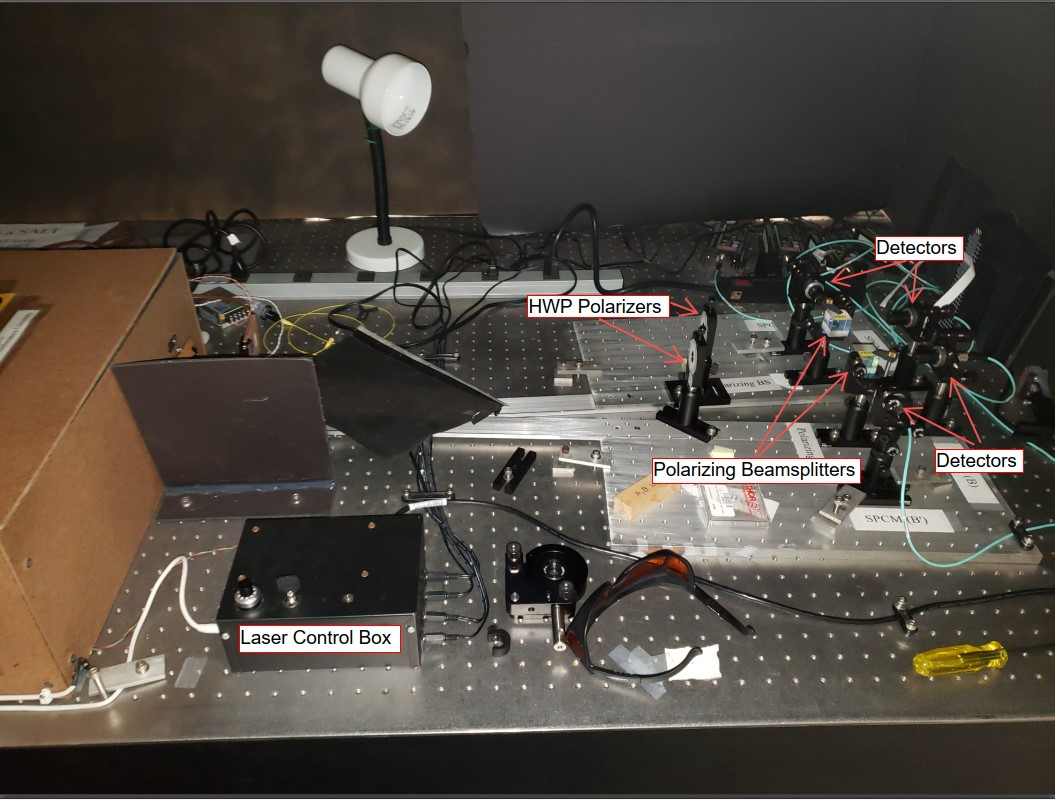
\includegraphics[width = 0.95\linewidth]{apparatus.jpg}
    \caption{The apparatus (labeled) used for this lab}
    \label{fig:app}
\end{figure}
The design of our apparatus has the purpose of creating entangled photons via a parametric down-conversion source (in our case, by using a pair of BBO crystals). Furthermore, this apparatus is also designed to be able to both count the number of photons that are transmitted/reflected from a 50/50 beamsplitter as well as count the number of coincidences from the signal and idler beams. 

We used a $405 \ \si{ nm }$ diode laser paired along with two BBO crystals (see Figure \ref{fig:laser}), which is what allowed for us to use utilize a Type-I down-conversion process. As noted in the Theory section of this lab report, this means that we will end up with two beams (signal and idler) that are polarized parallel to each other, with their polarization being perpendicular to that of the source/pump. Furthermore, we have that the wavelength of the photons in both of these beams to be double that of the diode laser -- i.e., we expect the signal and idler photons to have a wavelength of $810 \ \si{nm}$. It can be seen in Figure \ref{fig:app} that our apparatus is set up so that the signal and idler beams make a small angle with respect to the source/pump beam; doing so separates both beams so that they can be directed to their own 50/50 beamsplitter.
\begin{figure}[H]
    \centering
    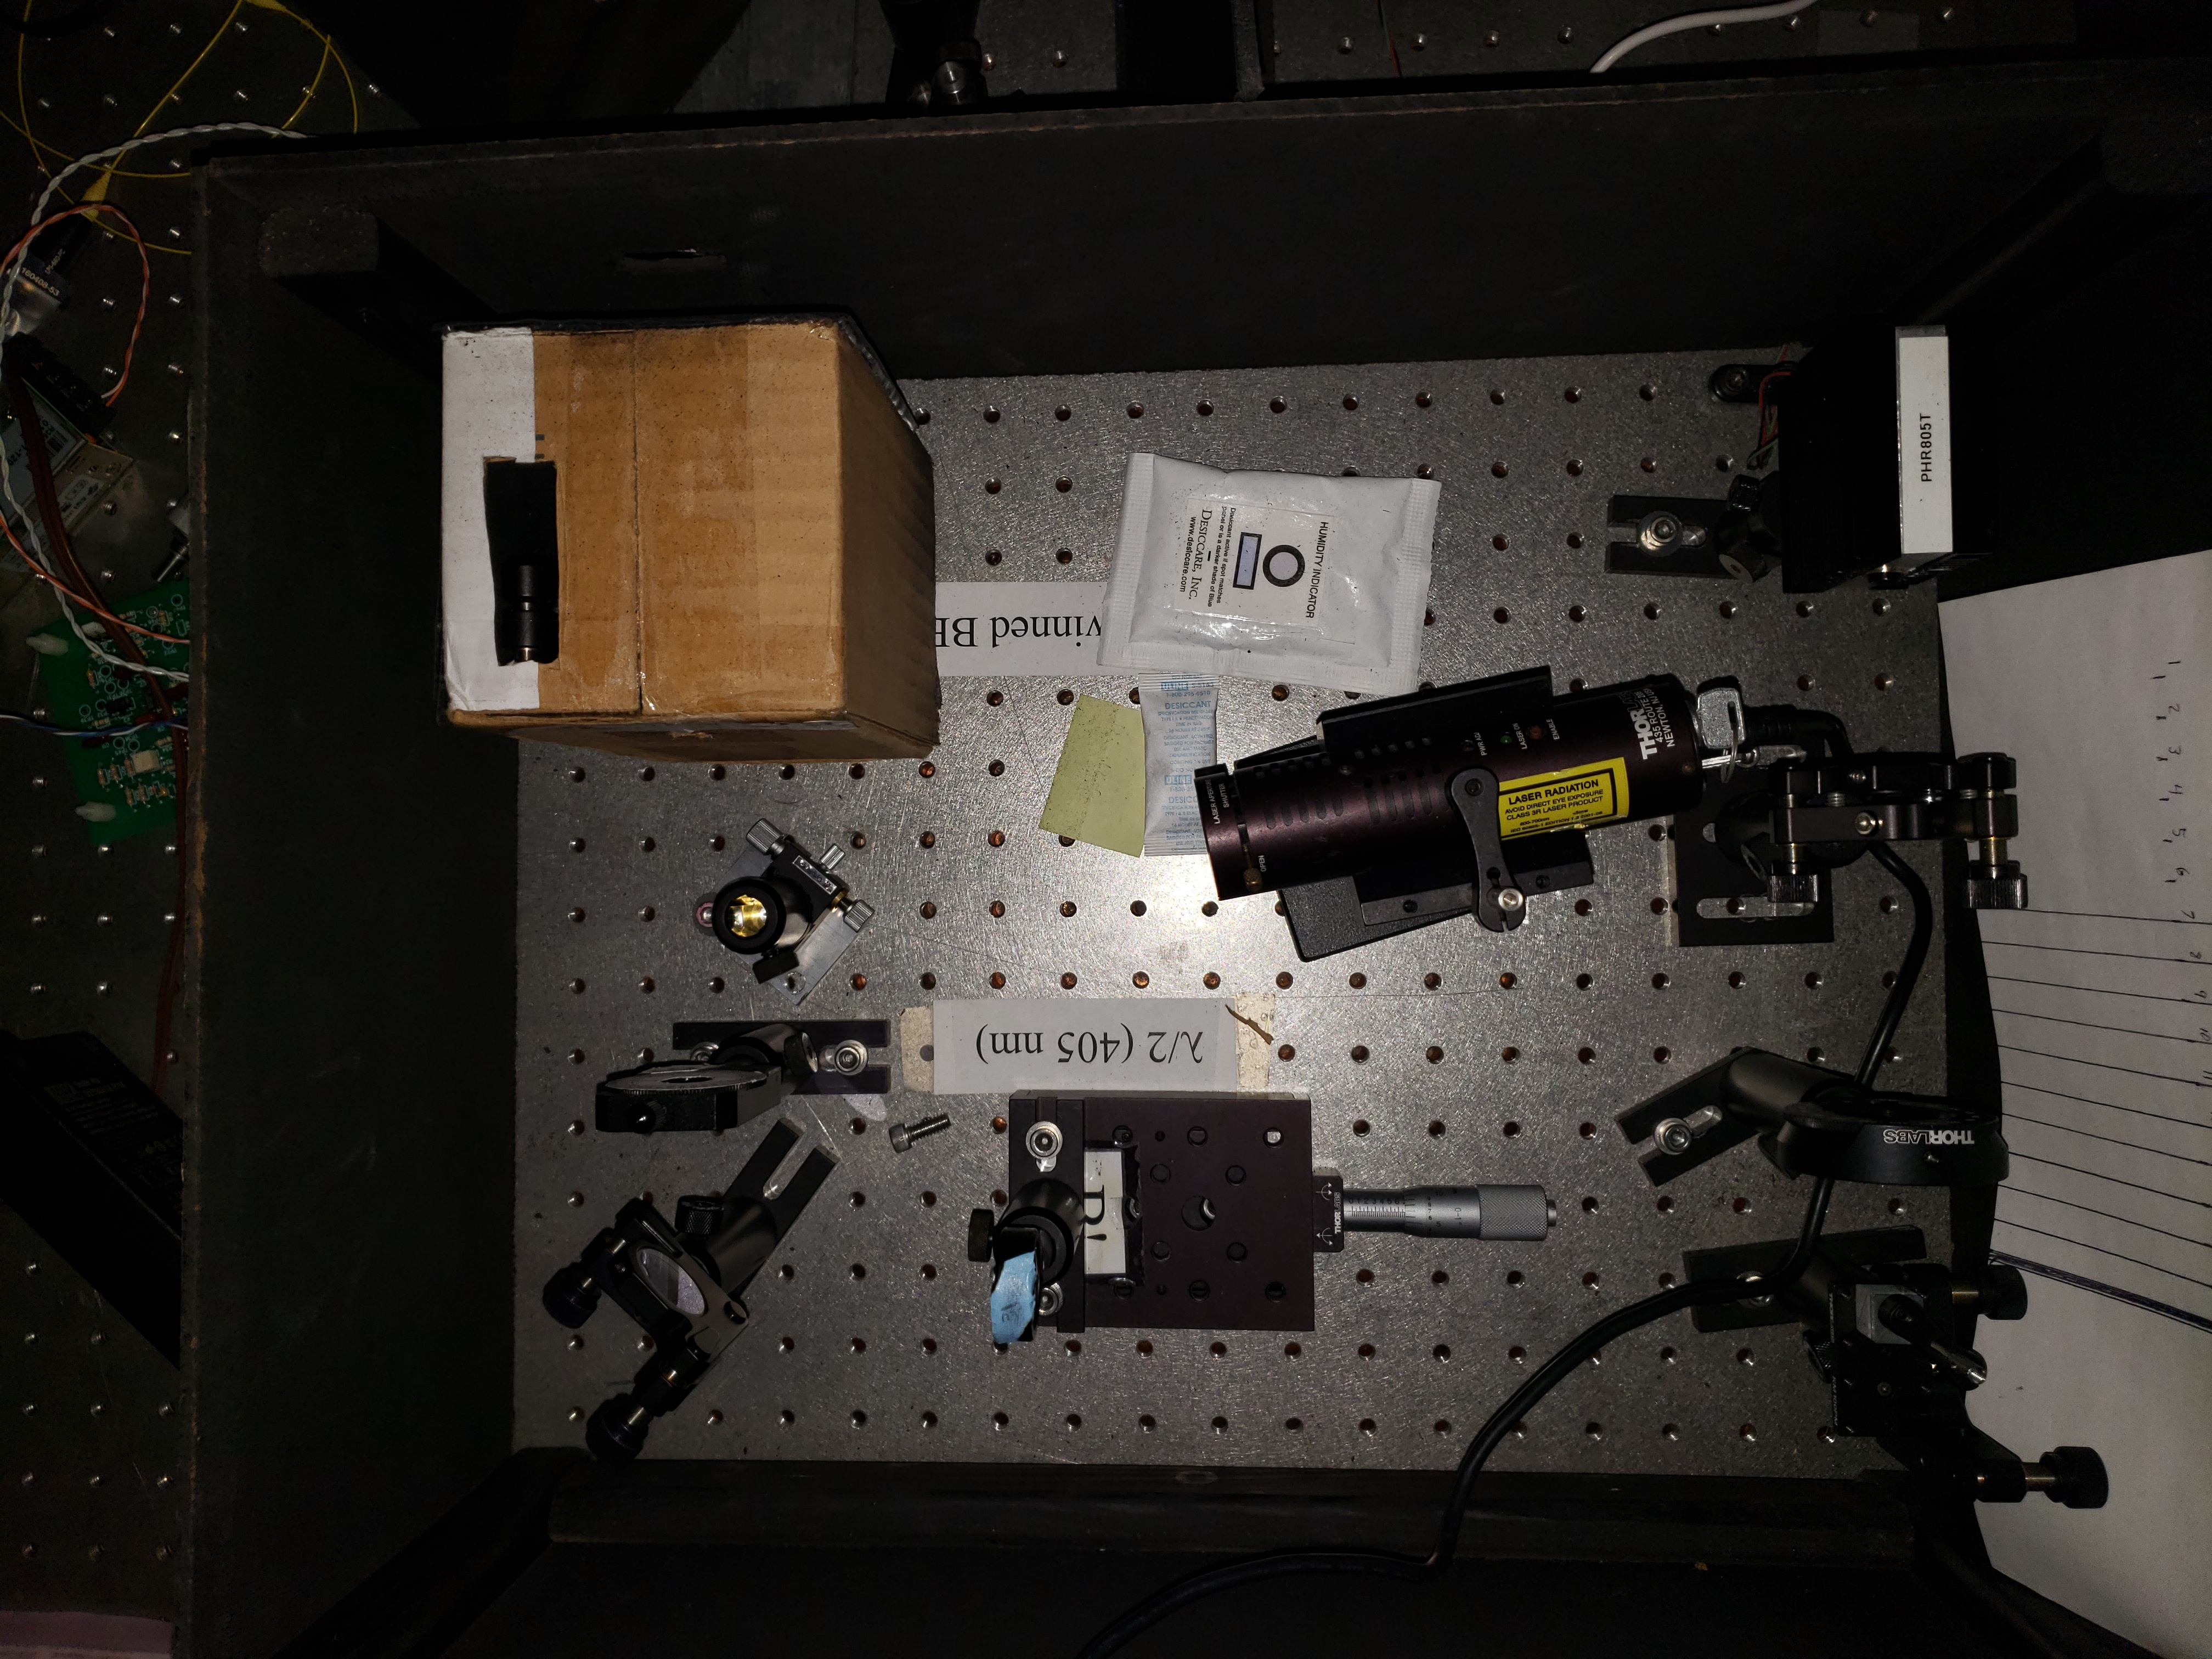
\includegraphics[width = 0.95\linewidth]{laser.jpg}
    \caption{The laser as well as the BBO crystals (inside the box in the upper-right corner) used for this lab.}
    \label{fig:laser}
\end{figure}

It can be seen in in Figure \ref{fig:app} that the transmitted/reflected signal and idler beams are directed towards detectors which will provide us with the number of photons detected. In particular, all the detectors we used for this lab are Excelitas' SPCM-AQRH Single Photon Counting Module -- more information on this detector can be found here \cite{photon_counting}. 

\begin{figure}[H]
    \centering
    \includegraphics[width = 0.95\linewidth ]{coincidence_counter.jpg}
    \caption{This device is what allowed for us to detect coincident counts between the two signal and idler beams}
    \label{fig:coincidence counter}
\end{figure}

On top of the detectors, we also made use of the device shown in Figure \ref{fig:coincidence counter}; this device allowed for us to detect coincident counts between the two signal and idler beams. Full details on how this device works and was built can be found here \cite{coincident_counter}. 

Also seen in Figure \ref{fig:app} are the HWP polarizers that are placed in front of the 50/50 beamsplitters. The function of these polarizers is that they allow for us to adjust the polarization of the incoming signal and idler beams before they reach the 50/50 beamsplitter. This function is vital towards our goal of disproving the HVT through the approach described in Dehlinger and Mitchell's paper \cite{D_M}.

Finally, the only part of the apparatus that is now shown in any of the figures is the program that we used to both view and collect the detected counts (including coincident) -- this being the LabView program. The program as well as its documentation can be found here \cite{labview}.

\section{Measurements and Data Analysis}

\subsection{Data Collection}
\subsubsection{Calculating the Second-Order Coherence $g^{(2)}(0)$}
Before we went about making any measurements or calculations, we observed the spontaneous parametric down-conversion by first properly aligning the BBO crystal. It should be noted that the BBO crystal was already aligned for us by the instructors of this lab. However, we needed to verify the alignment by checking if there is indeed spontaneous down-conversion happening. This could be done by using the LabView program and seeing whether or not there is an anticorrelation in the photocounts; to be explicit, we needed to check that if $N_{A}$ (or $N_{B}$) went up, then $N_{A'}$ (or $N_{B'}$) would go down and vice-versa. 

After we verified and observed the spontaneous parametric down-conversion, we then used the LabView program to gather all the necessary measurements to measure $g^{(2)}(0)$; these being $N_{A}, N_{AB}, N_{AB'},$ and $N_{ABB'}$. The structure of how we took our measurements is as follows: we took a total of 10 trials, where each trial consisted of 10 runs (each being 1 minute long). For each run, the LabView program provided the values of $N_{A}, N_{AB}, N_{AB'},$ and $N_{ABB'}$ for said run. With these values, all that was left was to calculate the value of $g^{(2)}(0)$.

\subsubsection{Violating the Bell Inequality}
As mentioned in the Introduction and Theory sections of this lab manual, the goal of this part of the lab is to disprove the HVT; Bell was able to do so by first obtaining an inequality that all HVTs must obey, and then showed that such an inequality was violated by quantum mechanics. In our case, the inequality that we will be using as our "Bell inequality" constrains the degree of polarization correlation under measurements at different polarizations; as mentioned before in the Bell Inequality section of this lab report, such an inequality was due to Clauser, Horne, Shimony, and Holt. As a recap of that section, we have that $S \leq 2$ for any HVT and arbitrary polarizer angles $a, a', b, b'$. 

In that section as well, we hinted that quantum mechanics can violate the inequality (that is, we can obtain $S > 2$), but only under certain settings.
One such setting (cleverly chosen by Dehlinger and Mitchell \cite{D_M}) would be when $a = 45^{\circ}$, $a' = 0^{\circ}$, $b = 22.5^{\circ}$, and $b' = -22.5^{\circ}$. As shown in their paper, it can be found that our value of $S$ using the HVT, denoted as $S^{(HVT)}$, with their choice of $a, a', b, b'$ maximizes our value; that is, we have $S^{(HVT)} = 2$. However, they also show in their paper that the value of $S$ using quantum mechanics, denoted as $S^{(QM)}$, with the same choice of $a, a', b, b'$ results in $S^{(QM)} = 2 \sqrt{2}$. It should be noted that this result is specific to the state $\vert \psi_{EPR} \rangle$, and that other states give lower values of $S$.

Thus, to achieve our goal of disproving the HVT, all we needed to do was to obtain/calculate a measurement of $S$ such that $S > 2$. This meant that we needed to calculate $E(\alpha, \beta)$ at the various polarizer angles $a = 45^{\circ}$, $a' = 0^{\circ}$, $b = 22.5^{\circ}$, and $b' = -22.5^{\circ}$ (the specific combinations of polarizer angles being given in Eqn. \ref{eq:S}). To obtain these polarizer angles, we used two HWP polarizers that were placed in front of each beamsplitter. 

However, the calibration of our HWP polarizers were off, meaning that we had to find the angle $\theta_{0}$ that corresponded to a polarizer angle of $0^{\circ}$ for both of them. This was done by first setting both HWP polarizers to their labeled angle of $0^{\circ}$ (again, this labeled angle did not match with the actual polarizer angle) and measuring $N_{A}, N_{A'}, N_{B}$, and $N_{B'}$ using the LabView program. We then adjusted the labeled angle to $40^{\circ}$ for both HWP polarizers and made the same type of measurements, and we repeated this process (adjusting the labeled angle by $40^{\circ}$ each time) until we obtained measurements for the entire $360^{\circ}$ range of the HWP polarizers. From this data, we were able to obtain the value of $\theta_{0}$ for each of the HWP polarizers by fitting our data accordingly -- this part will be discussed more in detail in the Data Analysis section. 

Once the HWP polarizers were calibrated, we then measured $N_{AB}, N_{A'B'}, N_{A'B}$, and $N_{AB'}$ using the LabView program at the various polarizer angles $a = 45^{\circ}$, $a' = 0^{\circ}$, $b = 22.5^{\circ}$, and $b' = -22.5^{\circ}$ (making sure to take $\theta_{0}$ into account in the process). The structure of how we took measurements is as follows: for each combination of polarizer angles (the total amount of combinations being 4, where Eqn. \ref{eq:S} gives us the particular combinations), we took a total of 4 trials, where each trial consisted of 10 runs (each being 18 seconds long). With all these measurements, all that was left to do was to calculate the values of $E(\alpha, \beta)$, which then allowed for us to calculate $S$.

\subsection{Data Analysis}
\subsubsection{Calculating the Second-Order Coherence $g^{(2)}(0)$}
As noted in the Data Collection section, the LabView program provided the values of $N_{A}, N_{AB}, N_{AB'},$ and $N_{ABB'}$ for each of the runs that we did. Using Eqn. \ref{eq:g2_qm_num}, we were able to calculate the value of $g^{(2)}(0)$ for each run that we ran. On top of that, we also made sure to account for the accidental coincidence counts; we did so by utilizing Eqns. \ref{eq:N_AB'} to \ref{eq:N_ABB''}, and the corrected counts are found as follows: 
\begin{equation}
    \begin{aligned}
        N_{AB}^{cor}
        &= 
        N_{AB} - N_{AB}'
        \\[2mm]
        N_{AB'}^{cor}
        &= 
        N_{AB'} - N_{AB'}'
        \\[2mm]
        N_{ABB'}^{cor}
        &= 
        N_{ABB'} - N_{ABB'}'
    \end{aligned}
\end{equation}
In terms of doing the actual calculations, we imported all the data into a csv file, which we then extracted using the \texttt{pandas} package. The extracted data would be in contained in a \texttt{pandas.DataFrame} object, which allowed for us to then easily compute $g^{(2)}(0)$ for each of the runs using the standard methods provided by \texttt{pandas.DataFrame}.

\subsubsection{Violating the Bell Inequality}
As noted in the Data Collection section, we measured the values of $N_{A}, N_{A'}, N_{B}$, and $N_{B'}$ at the various labeled polarizer angles for each of our HWP polarizers. We focus our attention to just one of the HWP polarizers (WLOG, we let it be the one that corresponds to $N_{A}$ and $N_{A'}$). We create two plots: one being a plot of $N_{A}$ with respect to the labeled polarizer angle, and the other being a plot of $N_{A'}$ with respect to the labeled polarizer angle. Notice that this is equivalent to us plotting out the intensity of the laser with respect to the labeled polarizer angle since we know that intensity is proportional to the number of photons. Thus, we know that the plots in both instances should be of the form $\sin^{2}(\theta - \theta_{0})$ or $\cos^{2}(\theta - \theta_{0})$ -- in our case, we have that the plot with $N_{A}$ corresponds closely with $\sin^{2}(\theta - \theta_{0, A})$, and the plot with $N_{A'}$ corresponds closely with $\cos^{2}(\theta - \theta_{0, A'})$ (as expected in this case since we know that detectors $A$ and $A'$ are off by a phase of $\frac{\pi}{2}$). Furthermore, we expect to have $\theta_{0, A}$ to match $\theta_{0, A'}$. 

As for how we went about finding $\theta_{0}$, we used python to fit our data to their corresponding models. To expand on this point further, let us focus on the data pertaining to $N_{A}$. We recall that the plot of $N_{A}$ with respect to the labeled polarizer angle corresponded closely with $\sin^{2}(\theta - \theta_{0, A})$. Thus, we used python (namely, the \texttt{lmfit} package) to fit our data to the following model: $a \sin^{2}(\theta - \theta_{0, A}) + y$, where we see that we are fitting for the amplitude $a$, the phase $\theta_{0, A}$, and vertical shift $y$. The result of this fit can be shown in Figure \ref{fig:theta_0_fit}, and we repeated the process for the data pertaining to $N_{A'}$, $N_{B}$, and $N_{B'}$ (making sure to use their corresponding models for each one).
\begin{figure}
    \centering
    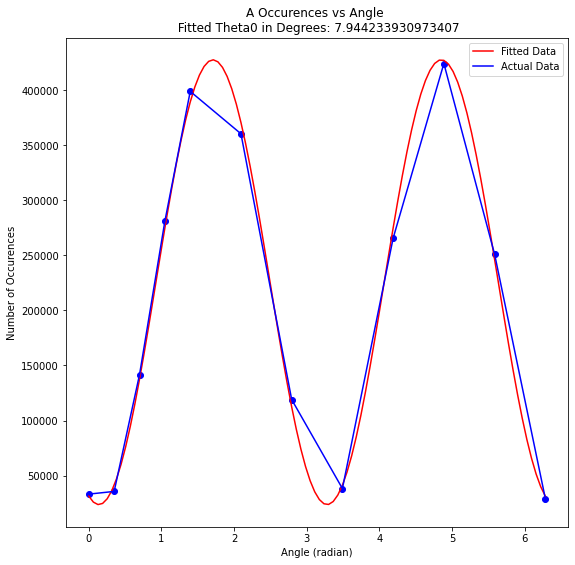
\includegraphics[width = 0.95 \linewidth]{theta_0.png}
    \caption{The fitted data pertaining to $N_{A}$ using the model equation $a \sin^{2}(\theta - \theta_{0, A}) + y$}
    \label{fig:theta_0_fit}
\end{figure}

After we obtained the values of $\theta_{0}$ for both HWP polarizers, we then moved onto obtaining measurements of $N_{AB}, N_{A'B'}, N_{A'B}$, and $N_{AB'}$. Once these were all gathered, we used Eqn. \ref{eq:E_num} to obtain a value of $E(\alpha, \beta)$ for each of the runs that we took. From these values of $E(\alpha, \beta)$, we then used Eqn. \ref{eq:S} to obtain a value of $S$; it should be noted that when calculating $S$, we did so as follows: for each combination of polarizer angles, we chose the values of $E(\alpha, \beta)$ in a corresponding manner -- that is, if we used the value of $E(a, b)$ that came from the first run of the first trial, then we shall use the values of $E(a, b')$, $E(a', b)$, and $E(a', b')$ that came the first run of the first trial as well.

Again, in terms of doing the actual calculations, we utilized the \texttt{pandas} package; we put all our data into a \texttt{pandas.DataFrame} object, and the standard methods provided by this object allowed for us to easily calculate $E(\alpha, \beta)$ for each run and $S$.

\subsection{Results}
\subsubsection{Calculating the Second-Order Coherence $g^{(2)}(0)$}
\begin{figure}[H]
    \centering
    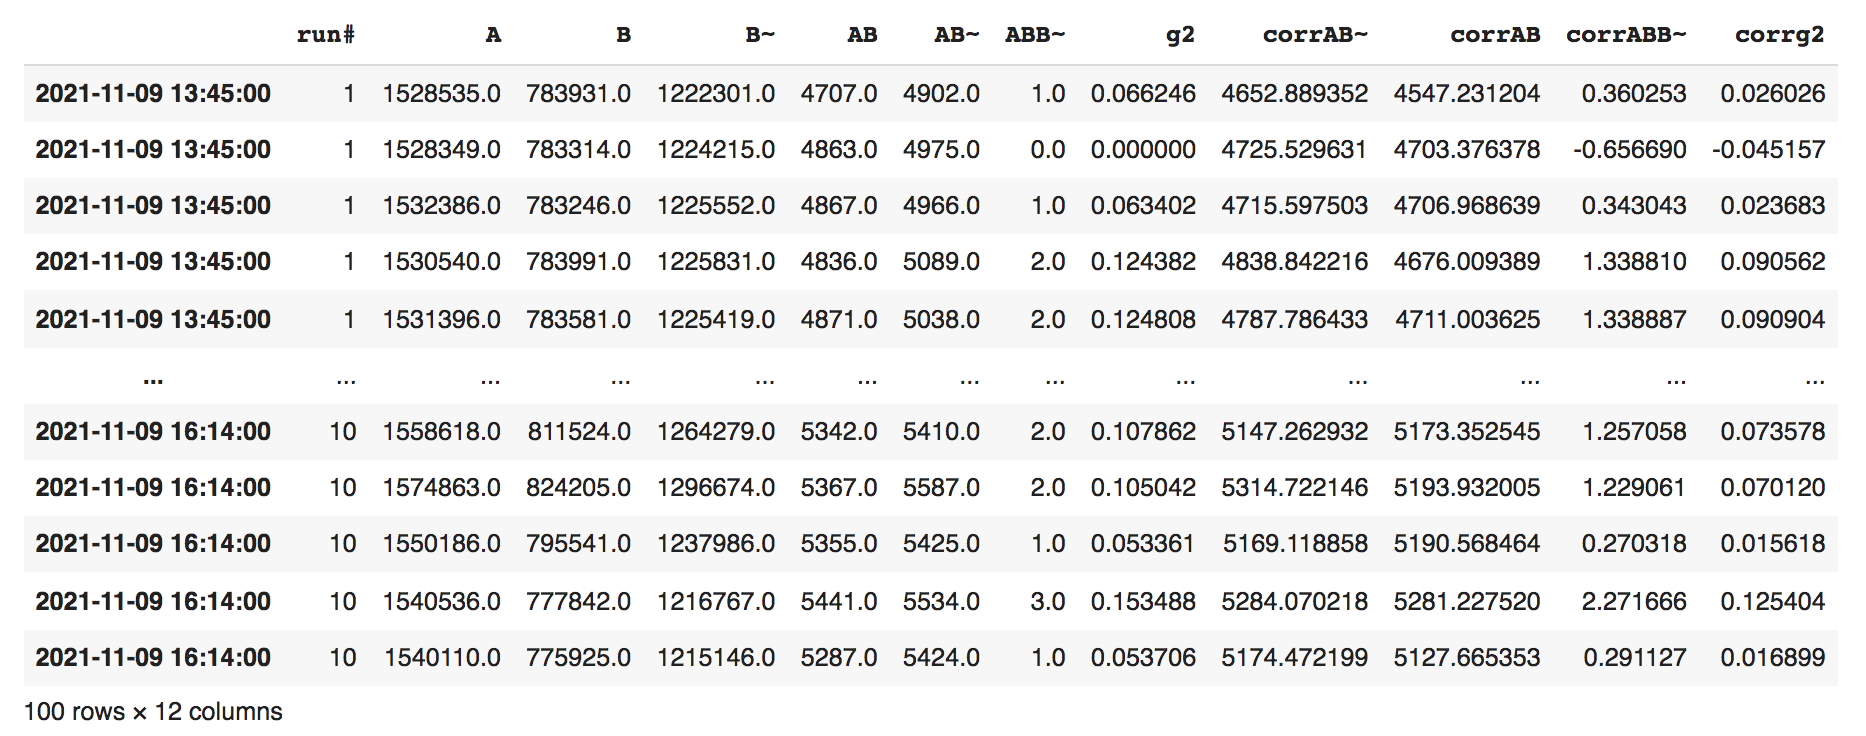
\includegraphics[width = 0.95\linewidth]{g2_table_values.png}
    \caption{A table of the calculated $g^{(2)}(0)$ values (includes the corrected values of $g^{(2)}(0)$ as well)}
    \label{fig:g2_table}
\end{figure}

Using the methodology described in the Data Analysis section, we were able to calculate the following value of $g^{(2)}(0)$
\begin{equation}
    g^{(2)}(0)
    =
    0.088 \pm 0.062
    \label{eq:calculated_g2}
\end{equation}
If we take into account the accidental coincidences, then we see that our corrected value of $g^{(2)}(0)$ is 
\begin{equation}
    g^{(2), cor}(0)
    =
    0.054 \pm 0.067
    \label{eq:calculated_g2_cor}
\end{equation}
The table that contains all the data can be found in Figure \ref{fig:g2_table}, and we also provide a histogram of the $g^{(2)}(0)$ and corrected $g^{(2)}(0)$ values in Figures \ref{fig:g2_hist} and \ref{fig:g2_hist_cor}, respectively.

\begin{figure}
    \centering
    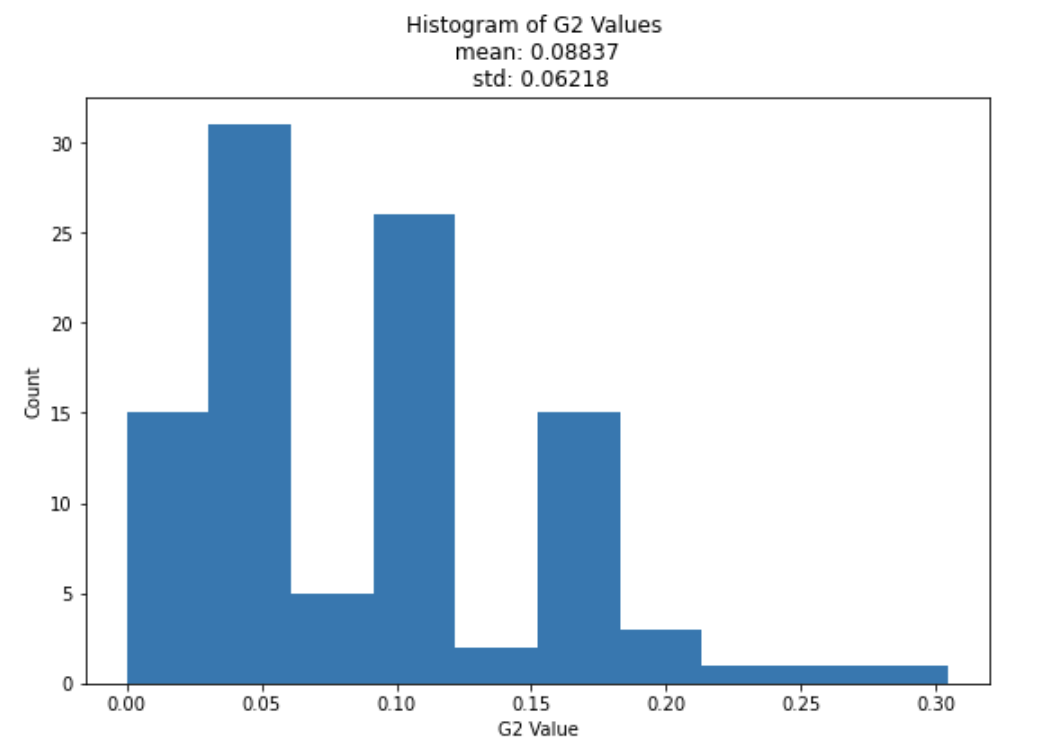
\includegraphics[width = 0.95\linewidth]{hist_g2.png}
    \caption{A histogram of the calculated $g^{(2)}(0)$ values }
    \label{fig:g2_hist}
\end{figure}

\begin{figure}
    \centering
    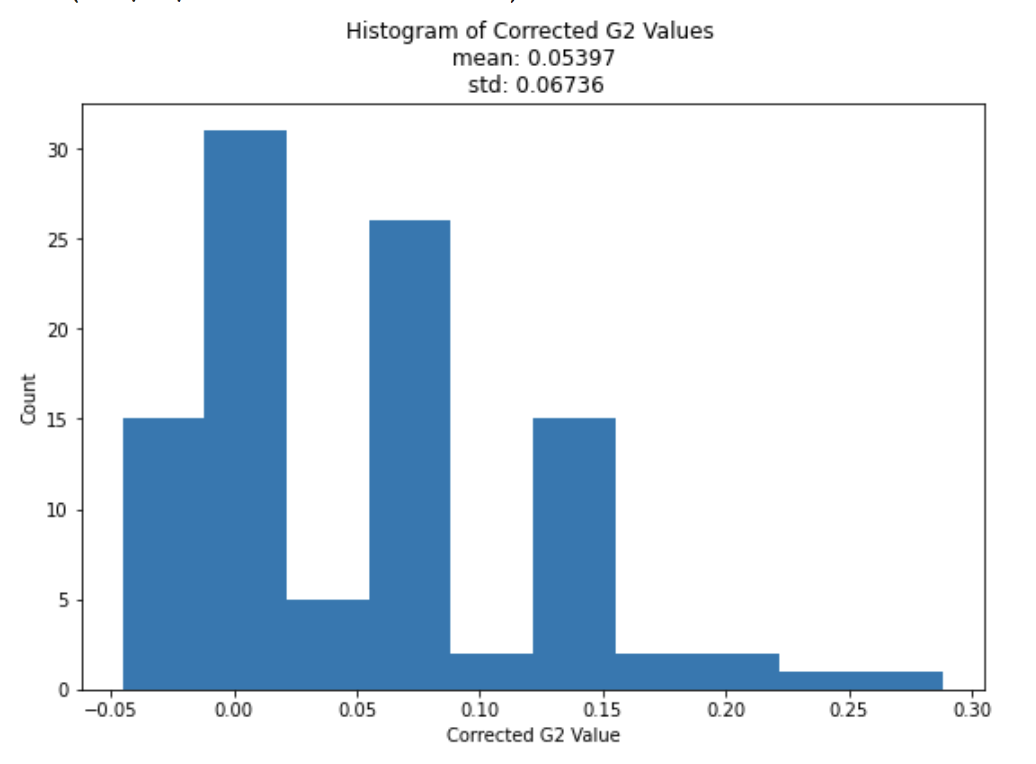
\includegraphics[width = 0.95\linewidth]{hist_g2_corrected.png}
    \caption{A histogram of the calculated corrected $g^{(2)}(0)$ values}
    \label{fig:g2_hist_cor}
\end{figure}

\subsubsection{Violating the Bell Inequality}
We start by noting that the data we collected/used in calibrating our HWP polarizers can be found in Figure \ref{fig:theta_0_data}.
\begin{figure}
    \centering
    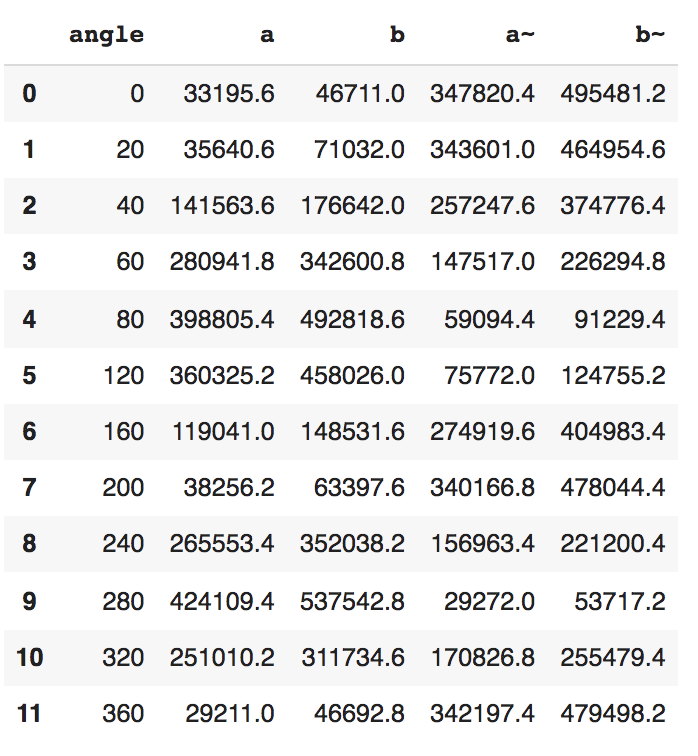
\includegraphics[width = 0.95 \linewidth]{theta_0_data.png}
    \caption{The number of photon detections for each of the detectors at various labeled polarizer angles (in degrees)}
    \label{fig:theta_0_data}
\end{figure}
As for the the fitted values of our phase angle $\theta_{0}$, we found the following values
\begin{center}
\begin{tabular}{||c | c||} 
 \hline
  & Fitted Phase Angle $\theta_{0}$ (in degrees)\\
 \hline
 $\theta_{0, A}$ & 7.9 \\ 
 \hline
 $\theta_{0, A'}$ & 8.3  \\
  \hline
 $\theta_{0, B}$ &7.7   \\
  \hline
 $\theta_{0, B'}$ & 7.6  \\
 \hline
\end{tabular}
\end{center}
Notice that there are no error bars for our fitted values of our phase angle $\theta_{0}$ in this case -- more on this will be discussed in the Discussion section of the lab report. 

We now move onto the data that we collected/used in calculating our value of $S$ as well as the calculated values of $S$ that we obtained; the data itself can be seen in Figure \ref{fig:S_data}, and our value of $S$ resulted to be 
\begin{equation}
    S
    =
    1.24 \pm 0.03
    \label{eq:S_value}
\end{equation}
A histogram of the calculated $S$ values can be found in Figure \ref{fig:S_hist}.

\begin{figure}
    \centering
    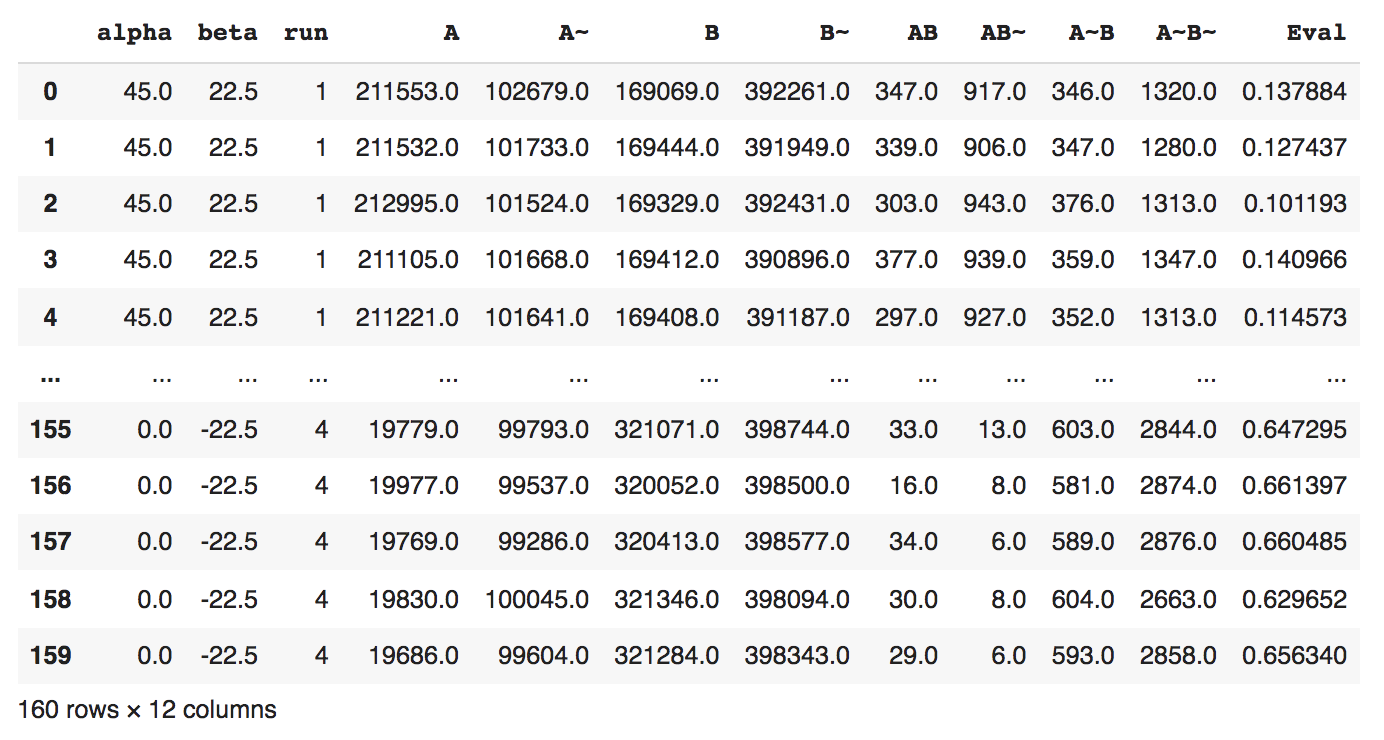
\includegraphics[width = 0.95 \linewidth]{S_data.png}
    \caption{The number of photon detections for each detector and coincident counts at various polarizer angle (in degrees) combinations}
    \label{fig:S_data}
\end{figure}

\begin{figure}
    \centering
    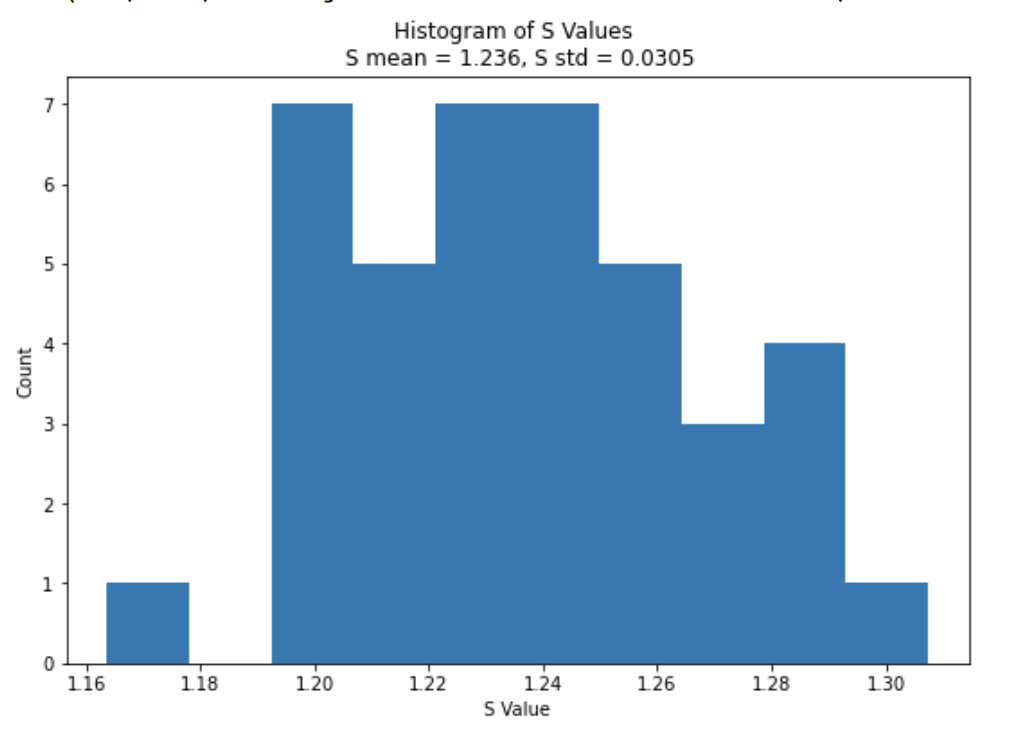
\includegraphics[width = 0.95 \linewidth]{s_hist.png}
    \caption{The histogram of the calculated $S$ values}
    \label{fig:S_hist}
\end{figure}

\section{Discussion}

\subsection{Discussion of Results}

\subsubsection{Calculating the Second-Order Coherence $g^{(2)}(0)$}
We can see from Eqns. \ref{eq:calculated_g2} and \ref{eq:calculated_g2_cor} that our values for $g^{(2)}(0)$ are much closer to 0 than they are to 1 -- which is consistent with what we expected to find. In fact, we can clearly see that our values of $g^{(2)}(0)$ in both cases are more than 6 standard deviations away from 1, which means that the classical field description is incorrect, and we have the QM descriptions of a field in a single photon state to match extremely well with our data. In short, we have shown that photons exist! 

We should note that we expect $g^{(2)}(0) = 0$ using the QM description of a field in a single photon state since we expect complete anticorrelation with such a description. This is because in the QM description of a field in a single photon state, it is impossible for us to obtain three-fold coincident count. Indeed, we do see from Eqns. \ref{eq:calculated_g2} and \ref{eq:calculated_g2_cor} that our values for $g^{(2)}(0)$ are within one standard deviation from the expected value of $g^{(2)}(0) = 0$, which tells us that our results are consistent with what we expected to find.

We now discuss the large error bars that are shown in the Eqns. \ref{eq:calculated_g2} and \ref{eq:calculated_g2_cor}; we start by noting that the equation that we used to calculate $g^{(2)}(0)$ (Eqn. \ref{eq:g2_qm_num}) is directly proportional to the three-fold coincident count $N_{ABB'}$. There were many instances where we did not obtain a three-fold coincident count, which meant that our calculated value of $g^{(2)}(0)$ resulted to be immediately 0, which then meant that our standard deviations were going to be large. 

\subsubsection{Violating the Bell Inequality}
We can see from Eqn. \ref{eq:S_value} that our calculated value of $S$ is less than 2, which is not consistent with what we expected to find. In fact, we can clearly see that our calculated value of $S$ is more than 6 standard deviations away from 2, which means that we can make no meaningful conclusion since we know that both HVTs and QM agree with this result. However, given the setup that we used, we expected $S < 2$, and we shall explain why in the Sources of Error section.

We now talk about why there were no error bars for our values of our phase angle $\theta_{0}$; in short, we were only able to gather enough data to find the fitted values of our phase angle $\theta_{0}$ once. If we had more time with the lab (each data collection session takes about 2 hours), then we would have taken more data, which would result in us getting multiple values for our phase angle $\theta_{0}$ -- thus, we would end up with error bars.

\subsection{Sources of Error}
When we calculated the values of $g^{(2)}(0)$, one possible source of error could have been from outside interference (that being of outside light). This would have resulted in false detections, which would skew our values for both the number of counts of the transmitted/reflection photons from the signal and idler beams as well as the coincident counts. Although we have accounted for accidental coincidences, we believe that this would not have accounted for all the possible false detections that we got from the outside interference. However, we should note that we tried our best to reduce the outside interference as much as possible by making sure that all light from our computers/other electronics as well as the light in the room was not incident on the detectors. With this considered, we believe that the effects from outside interference on our calculated value $g^{(2)}(0)$ to be small. 

Another source of error in calculating the values of $g^{(2)}(0)$ pertains to how we calculated the corrected value of $g^{(2)}(0)$. Looking at the histogram given in Figure \ref{fig:g2_hist_cor}, we can see that some values of $g^{(2)}(0)$ are negative when they should have been 0 instead. This was an error in how we calculated the corrected value of $g^{(2)}(0)$; in particular, we ended up with situations where $N_{ABB'} < N_{ABB'}'$, which meant that the corrected value of $N_{ABB'}$ would result to be negative. We should have instead set a lower bound of 0 for each of the corrected values to avoid this error.

Moving onto when we calibrated the HWP polarizers and calculating the values of $S$, we note that one source of error came from the lack of precision when setting the HWP polarizers to certain angles; to expand on this point, the spacing between the ticks on the HWP polarizers are $4^{\circ}$ apart, and these ticks were very hard to see and were very close to each other. As a result, this more than likely resulted in us incorrectly setting the polarizer angle a few times. Thus, we believe that this affected the fitted values of our phase angle $\theta_{0}$ and calculated value of $S$ by a non-negligible amount. However, we think that we could have reduced the effect significantly if we took the time to include error bars for when we set the polarizer angles (i.e., we would have error bars for $\theta$), and making sure to account for these error bars when we were fitting for the phase angle $\theta_{0}$ and calculating our values of $S$.

We also note that we calculated our values of $S$ without correcting for the accidental coincident counts; we realized this after looking at the code used for calculating such values, and we should have used the corrected values instead.

However, the largest source of error came from our laser.
As noted in both the Theory and Data Collection portion of the lab manual, getting a measured value of $S$ was reliant on our ability to produce entangled particles. It is here that we note that in order to create entangled particles, we must have a photon to interact with both of the BBO crystals -- however, our laser has such a short coherence time that it results in photons to almost never interact with both crystals. Thus, we are fairly confident that the particles that are being produced via the spontaneous parametric down-conversion are not entangled, which means that it is almost impossible to get the desired inequality of $S > 2$. 

\section{Conclusion}
In this lab, we were able to prove the existence of photons by comparing what we expect the second-order coherence $g^{(2)}(0)$ to be for a classical field description versus a QM field description of a single photon state; in short, we expect $g^{(2)}(0) \geq 1$ for a classical field description and $g^{(2)}(0) < 1$ for a QM field description of a single photon state. The importance of $g^{(2)}(0) < 1$ lies in the fact that such an inequality means that the transmitted and reflected detections must be anticorrelated, which happens when we are dealing with photons. We were able to show in Eqns. \ref{eq:calculated_g2} and \ref{eq:calculated_g2_cor} that our calculated values of $g^{(2)}(0)$ were consistent with what we expected, thus proving the existence of photons.

We then went about disproving the HVT; to do so, we had to violate a Bell inequality that pertained to the setup of our lab. One such Bell inequality was due to Clauser, Horne, Shimony, and Holt, and it told us that all HVTs must satisfy $S \leq 2$. It was through a clever choice of polarizer angles (found by Dehlinger and Mitchell) that they were able to maximize $S$ calculated using the HVT (i.e. $S^{(HVT)} = 2$), but showed as well that such choice of polarizer angles also resulted in $S$ calculated using QM to be $S^{(QM)} = 2 \sqrt{2} > 2$, which violated our Bell inequality. However, we were unable to violate such an inequality with the main reason being that our laser made it almost impossible to produce entangled photon pairs (which was required in obtaining $S > 2$).

As for possible ways to make the lab better, we start by noting that we could have a done the experiment in a more isolated setup -- one that completely reduces outside interference, which takes away the possibility of false counts occurring. Furthermore, the portion of the lab pertaining to violating the Bell inequality would have been done better if we have a more precise HWP polarizer to work with; this way, we could set the polarizer angles more precisely, which would result in more accurate values for our fitted value of our phase angle $\theta_{0}$ and our calculated value of $S$.

The most obvious way to improve the lab would be to use a better laser -- one that allows for the production of entangled photon pairs. Doing so would have increased our chances of obtaining $S > 2$ siginificantly. 

Finally, the last way that we could have improved our results was on how we calculated the value of $S$; the way we calculated it is as follows: for each combination of polarizer angles, we chose the values of $E(\alpha, \beta)$ in a corresponding manner -- that is, if we used the value of $E(a, b)$ that came from the first run of the first trial, then we shall use the values of $E(a, b')$, $E(a', b)$, and $E(a', b')$ that came the first run of the first trial as well. We realize that there are most likely better approaches to calculating $S$ than the approach that we took (perhaps, we could have used averages instead).

\bibliographystyle{unsrt}
\bibliography{References}
\end{document}